\chapter{Evaluation}
Evaluating visualizations is of paramount importance because it impacts how individuals, 
organizations, and societies interpret and make decisions based on data. Poorly designed 
visualizations can lead to misunderstandings, incorrect conclusions, and misguided 
decisions, whereas effective visualizations can facilitate better understanding, 
insights, and actions. In fields where data and decisions are critical—such as science, 
business, and public policy -- the ability to accurately and effectively visualize information 
is a powerful tool for communication and understanding.

\section*{Evaluating Visualizations with Usability Testing}
Usability testing is a popular User Experience research methodology that focuses on collecting
insights, findings, and anecdotes about how people view a visualization. In a usability-testing 
session or survey, a researcher asks participants to perform tasks and interpret specific visualizations
while observing the participant's behavior and listening to their feedback. Qualitative usability 
testing is best for discovering problems in the user experience and is more common than quantitative 
usability testing, which focuses on collecting metrics to describe the user experience.
It's important to perform such a survey with more than just one sample person as the goal mainly is to 
find overlapping and individual observations and patterns in the feedback which both can be used to either 
validate or improve a visualization \cite{nngroupUsabilityTestingUsers2018}.

In this report, these following two visualizations will be evaluated with a usability test (survey):
\begin{figure}[htb]%
    \centering
    \subfloat{{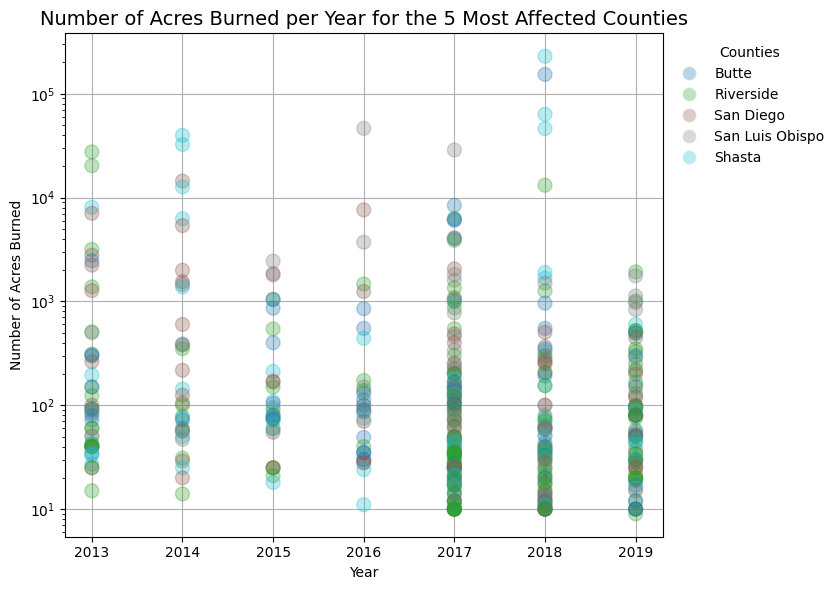
\includegraphics[width=.4\textwidth]{figures/survey_1.png} }}%
    \qquad
    \subfloat{{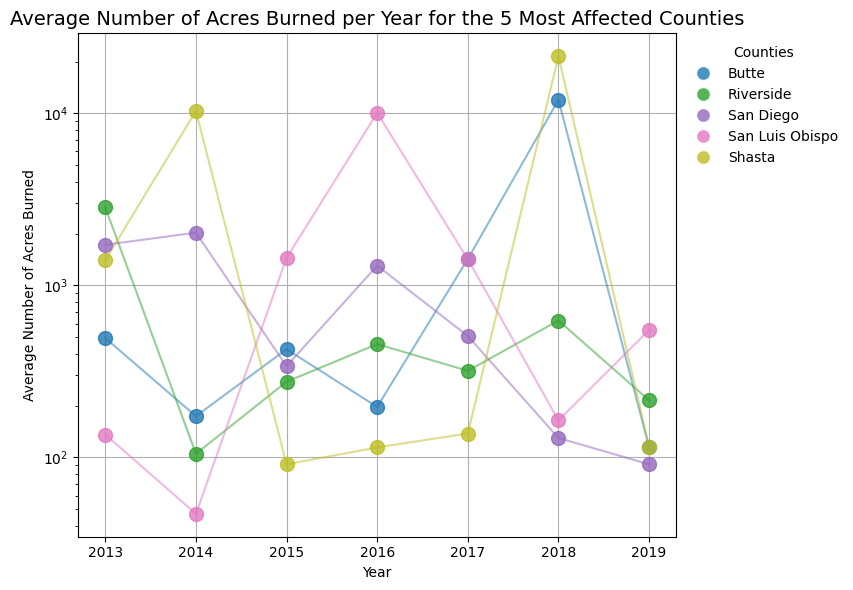
\includegraphics[width=.4\textwidth]{figures/survey_2.png} }}%
    \caption{Visualizations used in the Usability Test}%
    \label{fig:example}%
\end{figure}

\section*{Defining the Usability Test's Environment}
For the usability test of the visualizations, a cohort of five individuals from diverse backgrounds, ages 
and professions were selected to ensure a wide range of perspectives and experiences. 

The following questions were asked for both visualizations:
\begin{table}[H]
    \centering
    \begin{tabular}{|l|p{0.9\textwidth}|}
    \hline
    \textbf{\#} & \textbf{Question} \\ \hline
    1           & Which county seems to have been affected the most severe by fires? \\ \hline
    2           & Which year was the worst when it comes to wildfires? \\ \hline
    3           & Are there any elements or aspects of the visualization that confuse you? \\ \hline
    4           & Can you see a relationship between the year and the acres burned? \\ \hline
    5           & Can you see any pattern for a single county, if so what can you notice? \\ \hline
    \end{tabular}
    \caption{Usability Test Questions for Visualizations}
\end{table}

The questions were asked during a video call with the participants. The visualizations were given 
to the participants in random order but one at a time.

\section*{Analyzing the Results}
\subsection*{Question 1}
The first visualization consistently indicates that Butte County has been most severely affected by 
wildfires, particularly in the year 2018. This observation is clear for 4 of the 5 subjects, 
showing that the visual distinction of Butte County's data is effectively communicated in the design.
However subjects that elaborated on the second visualization correctly noted that it is not clear which 
county was most affected as the data points got averaged.

\subsection*{Question 2}
All subjects identified 2018 as the year with the most significant impact from wildfires in both visualizations.
This validates the visualizations' effectiveness in conveying temporal trends and highlighting outlier 
events, which is crucial for understanding the temporal scope of the data.

\subsection*{Question 3}
4 of 5 subjects noted potential confusion arising from the log scale on the y-axis and the overlapping 
data points in the first visualization. The second visualization's line graph was also noted to potentially 
imply continuity where there is none. Thus, these points resemble areas for design refinement to enhance the 
clarity and a more intuitive understanding. All five subjects struggled with the question when looking at how
much time they needed -- An observation that seems to have caused this was that most of the subjects were 
trying tell what number was lying beneath the y-scale.

\subsection*{Question 4}
The relationship between the year and the number of acres burned is not consistently apparent across subjects, 
with some recognizing an increasing trend, while others see variability. 3 of the 5 subjects tried to name a trend
by mainly looking at the connecting lines in the second visualization. The goal of the lines between the scatters
was to make it easier to follow each county over time -- This seems to have caused confusion and would need to be
improved in a future iteration. 

\subsection*{Question 5}
Patterns within single counties were observed differently by all subjects, with some noticing fluctuating trends 
and others identifying specific years of extreme wildfire activity. The variance in interpretation leads to the fact 
that while individual events are highlighted effectively, the overall pattern communication could be improved 
to ensure consistent comprehension among all viewers.

\subsection*{Summary}
The goal with these visualizations was to convey the severity of wildfires in California for the biggest counties.
All of the subjects were focusing on the actual number of acres which were burned and not the overall trend and 
severity. The biggest reason for that contextual misunderstanding was the log scale on the y-axis.
The extremes were pointed out correctly by all subjects and a trend was not falsely identified by anyone.